% figures/detect/fig_manifold.tex — loads PDF exported from NB03/NB05
% Requires \usepackage{graphicx}. Export the PC1-PC2 latent cloud
% (and/or the AE-vs-PCA comparison) as figures/detect/manifold.pdf.
\begin{figure}[!ht]
    \centering
    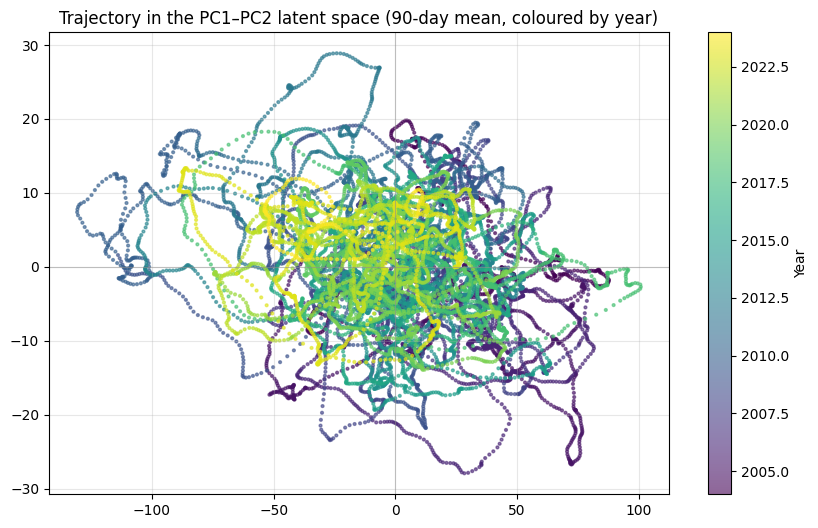
\includegraphics[width=0.85\textwidth]{figures/data_pipeline/fig_manifold.png}
    \caption[The flat latent manifold of AMOC profiles.]{\textbf{The manifold of
    AMOC vertical profiles is flat.} Each point is one day, placed by its two
    latent coordinates --- PC1 (intensity) and PC2 (vertical redistribution). A
    non-linear autoencoder trained on the same profiles reconstructs them no
    better than linear PCA at any latent dimension (gap $-0.06$ to $-0.15$
    percentage points; see Table~\ref{tab:ae-gap}), confirming that two straight
    coordinates capture the structure without distortion.}
    \label{fig:manifold}
\end{figure}
